\documentclass{beamer}
%\documentclass[handout]{beamer}

\mode<presentation>
{
%  \usetheme{Warsaw}
  % or ...

%  \setbeamercovered{transparent}
  % or whatever (possibly just delete it)
}


\setbeamertemplate{navigation symbols}{}

\usepackage[utf8]{inputenc}
\usepackage[spanish, es-tabla, es-nodecimaldot]{babel}
\usepackage{xcolor}


%\usepackage{times}
%\usepackage[T1]{fontenc}
% Or whatever. Note that the encoding and the font should match. If T1
% does not look nice, try deleting the line with the fontenc.


\title[Intro Prog] % (optional, use only with long paper titles)
{Introducción a la programación}

\subtitle
{Usando Python}

\author[MS]
{Mateo Suster \\ mateosuster@gmail.com}%\inst{1}}
% - Give the names in the same order as the appear in the paper.
% - Use the \inst{?} command only if the authors have different
%   affiliation.

\institute[UNGS] % (optional, but mostly needed)
{
%  \inst{1}%
  Matemática para Economistas III \\ 
  Instituto de Industria\\
  Universidad Nacional de General Sarmiento
%  \and
%  \inst{2}%
%  Department of Theoretical Philosophy\\
%  University of Elsewhere}
% - Use the \inst command only if there are several affiliations.
% - Keep it simple, no one is interested in your street address.
}

\date[] % (optional, should be abbreviation of conference name)
{ \today}



% If you have a file called "university-logo-filename.xxx", where xxx
% is a graphic format that can be processed by latex or pdflatex,
% resp., then you can add a logo as follows:

% \pgfdeclareimage[height=0.5cm]{university-logo}{university-logo-filename}
% \logo{\pgfuseimage{university-logo}}



% Delete this, if you do not want the table of contents to pop up at
% the beginning of each subsection:
%\AtBeginSubsection[]
%{
%  \begin{frame}<beamer>{Outline}
%    \tableofcontents[currentsection,currentsubsection]
%  \end{frame}
%}


% If you wish to uncover everything in a step-wise fashion, uncomment
% the following command: 

%\beamerdefaultoverlayspecification{<+->}


\begin{document}

\begin{frame}
  \titlepage
\end{frame}


\begin{frame}{Antes de arrancar...}
%  \tableofcontents
  % You might wish to add the option [pausesections]
  \begin{block}{Algunas pautas de (esta parte de) la materia}
  \end{block}\pause
  \begin{itemize}
  	\item Todas las preguntas son válidas. \pause Además, las buenas preguntas son más importantes que las buenas respuestas. \pause
	\item Es importante ir practicando (poco a poco) las cosas que vamos a ir viendo. \pause Esto permitirá evitar la \emph{montaña} de fin de cuatrimestre. \pause (¿Qué necesito para esto?) \pause
	\item Canales de comunicación: \pause Slack (preferentemente) o mail (en casos más puntuales). \pause
	\item Instancias de evaluación \pause
		\begin{itemize}
			\item Participar en Slack (preguntando, respondiendo, debatiendo, "molestando", etc.) \pause
			\item Trabajos Prácticos cuasi-semanales (sin patrón de repetición)\pause
			\item Exámenes Parciales (1 ó 2; fechas a definir)
		\end{itemize}	
  \end{itemize}
\end{frame}

\begin{frame}{Evitar la "montaña" de fin de cuatrimestre} \pause
\begin{center}
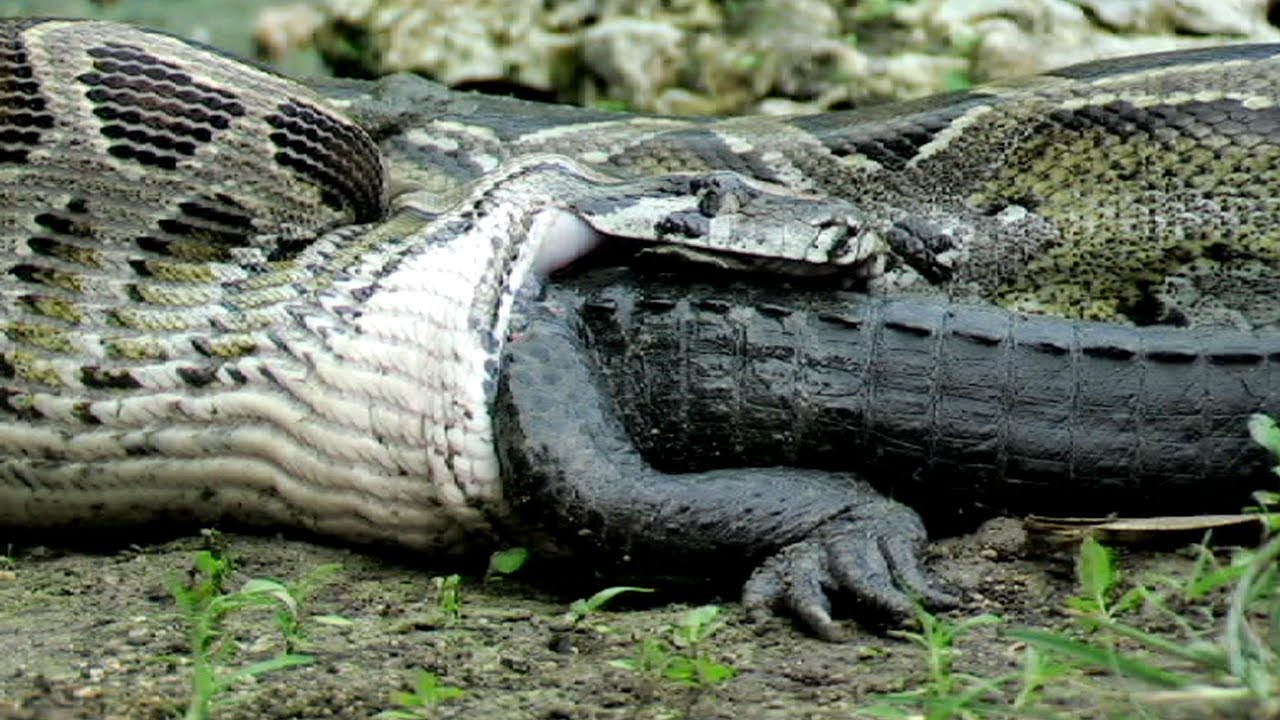
\includegraphics[height=5cm, scale=0.5]{recursos/eat_alligator.jpg}
\end{center}
\end{frame}

\begin{frame}{Introducción}
%  \tableofcontents
  % You might wish to add the option [pausesections]
  \begin{block}{Info general:}

  \end{block}\pause
  \begin{itemize}
  	\item Objetivo (en principio): programar un sistema de EDOs y graficarlo.
	\pause
	\item Objetivo (en el fondo): generar habilidades que los introduzcan de manera autodidáctica en el mundo de la programación \pause
	\item ¿Qué es programar? \pause
		\begin{itemize}
			\item Programar $\neq$ saber un lenguaje de programación. \pause
			\item Programar $\neq$ saber usar una computadora. \pause
			\item Frase de Edgar Dijkstra: ``La Ciencia de la Computación no tiene que ver con las computadoras más que la Astronomía con los telescopios''.\pause
		\end{itemize}
	\item ¿Qué lenguajes de programación conocen?\pause
	\item ¿Cuál lenguaje vamos a usar nosotros?\pause
	\begin{itemize}
		\item Respuesta corta: Python. \pause
		\item Respuesta larga: no importa demasiado. Lo importante  son los conocimientos básicos de programación, que son comunes a la mayoría de los lenguajes.%\pause
	\end{itemize}
  \end{itemize}
\end{frame}

\begin{frame}{¿Pero entonces porqué Python?} \pause
\begin{block}{Python actualmente es muy popular}  \pause
	\begin{itemize}
		\item Veamos el \textcolor{blue}{\href{https://www.tiobe.com/tiobe-index/}{Índice Tiobe}}
	\end{itemize}
\end{block}
\begin{center}
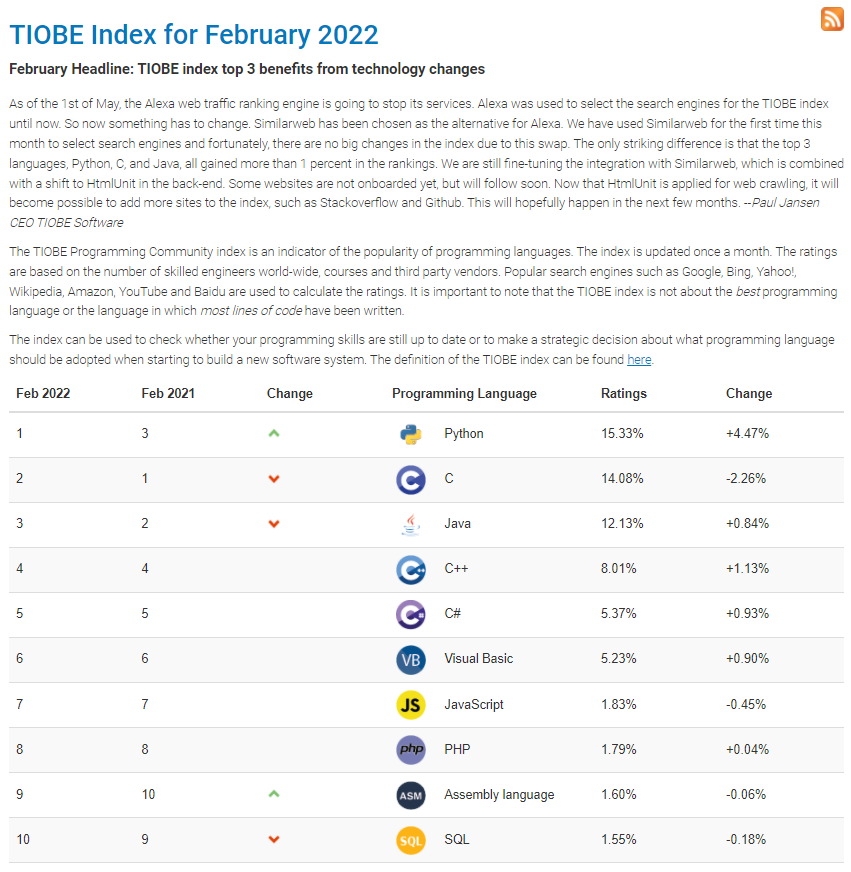
\includegraphics[height=7cm, scale=0.5]{recursos/tiobe_index22.png}
\end{center}
\end{frame}

\begin{frame}{Más ventajas de Python} \pause
\begin{itemize}
	\item Lenguaje \textcolor{blue}{\href{https://www.computerweekly.com/es/definicion/Programacion-orientada-a-objetos-OOP}{orientado a objetos}} relativamente "fácil" de aprender (\textcolor{blue}{\href{https://www.diarlu.com/lenguajes-de-programacion/}{lenguaje de alto nivel}}) \pause
	\item Enfoque simple y sintaxis elegante: su lenguaje enfatiza la sencillez de código y legibilidad \pause
	\item Poderosa capacidad de cómputo \pause
	\item Open Source Software (código abierto) \pause	
	\item Aplicaciones en diversas áreas. Hoy en día, se utiliza en la mayoría de las \textcolor{blue}{\href{https://learn.onemonth.com/es/10-paginas-web-famosas-hechas-con-python/}{plataformas que conocemos}} y tiene un extendido uso en la Ciencia de datos (en todos sus "componentes", como la Estadística, el Aprendizaje Automático, la Inteligencia Artificial (IA), Data Mining, etc. etc, todos los cuales entran en lo que se conoce popularmente como Big Data).
\end{itemize}
\end{frame}


\begin{frame}{¿Sólo por eso elegimos Python?} \pause
Hay otro motivo... \pause
\begin{center}

\includegraphics[height=7cm, scale=0.5]{recursos/yoda.png}
\end{center}
\end{frame}


\begin{frame}{Recursos Python}
(\footnotesize Están también en la página \url{https://sebasped.github.io/pythonungs/})
\begin{itemize}
	\item Comunidades:
	\begin{itemize}
		\item \footnotesize\url{http://www.python.org.ar/}
		\item \footnotesize\url{https://argentinaenpython.com/}
		\item \footnotesize\url{https://twitter.com/ChicasProgAR}
		\item \footnotesize\url{https://www.chicasentecnologia.org/}
		\item \footnotesize\url{https://twitter.com/lasdesistemas}
		\item \footnotesize\url{https://www.meetup.com/Buenos-Aires-Python-Meetup/}
		\item \footnotesize\url{https://twitter.com/linuxchixar}
	\end{itemize}\pause
	\item Material, cursos, tutoriales, bibliografía:
	\begin{itemize}
		\item Tutorial de Python para no programadores: \footnotesize\url{http://jjc.freeshell.org/easytut/easytut_es/easytut.html}
		\item \footnotesize\url{http://www.python.org.ar/wiki/AprendiendoPython}
		\item \footnotesize\url{https://argentinaenpython.com/quiero-aprender-python/aprenda-a-pensar-como-un-programador-con-python.pdf}
		\item \footnotesize\url{https://launchpadlibrarian.net/18980633/Python\%20para\%20todos.pdf}
		\item Cursos online (en inglés): coursera, datacamp, udemy, Stanford online, edx, codeacademy, Harvard online, etc.
		%		\item Pilas, colas.
	\end{itemize}\pause
	\item Buscar en internet: hay mucho mucho hecho ya.
\end{itemize}
\end{frame}



\begin{frame}{Elementos básicos programación} \pause
\begin{itemize}
	\item Diferencia entre algoritmo y programa.\pause
	\item Herramientas esenciales:
	\begin{itemize}
		\item Tipos de datos: enteros, reales, strings, etc.% \pause
		\item Variables y expresiones.% \pause
		\item Instrucciones: asignación, condicional, ciclo.%\pause
		\item Funciones, pasajes de parámetros.
	\end{itemize}\pause
	\item Estructuras de datos:
	\begin{itemize}
		\item Listas, arreglos.
		\item Conjuntos, diccionarios.
		\item Pilas, colas.
		\item DataFrames
	\end{itemize}\pause
	\item ¿Cómo se aprende a programar? \pause Programando... no hay manera de aprender algo sin hacerlo.
\end{itemize}
\end{frame}




\begin{frame}{Algoritmo} \pause
\begin{itemize}
	\item Un \emph{algoritmo} es una secuencia de instrucciones. Por ejemplo:\pause
		\begin{enumerate}
		\item Moje el cabello. \pause
		\item Coloque champú.\pause
		\item Masajee suavemente y deje actuar por 2 min.\pause
		\item Enjuague. \pause
		\item Repita el procedimiento desde 1.
		\end{enumerate}
\end{itemize}
\end{frame}

\begin{frame}{Algoritmo}
\begin{itemize}
	\item Una instrucción es una operación que:
	\begin{itemize}
		\item \textcolor{green}{transforma los datos}, o bien
		\item  \textcolor{red}{modifica el flujo de ejecución}
	\end{itemize} \pause
\end{itemize}	
	
		\begin{enumerate}
		\item \textcolor{green}{Moje el cabello.}% \pause
		\item \textcolor{green}{Coloque champú.}% \pause
		\item \textcolor{green}{Masajee suavemente} y \textcolor{red}{deje actuar por 2 min.}%\pause
		\item \textcolor{green}{Enjuague}.
		\item \textcolor{red}{Repita el procedimiento desde 1.}
		\end{enumerate}

\end{frame}




\begin{frame}{Programa} \pause
	\begin{itemize}
	\item Un \emph{programa} es una implementación de un algoritmo en un lenguaje de programación. \pause
		\begin{itemize}
		\item El programa representa al algoritmo en el lenguaje. \pause
		\item Las instrucciones son propias del lenguaje.
		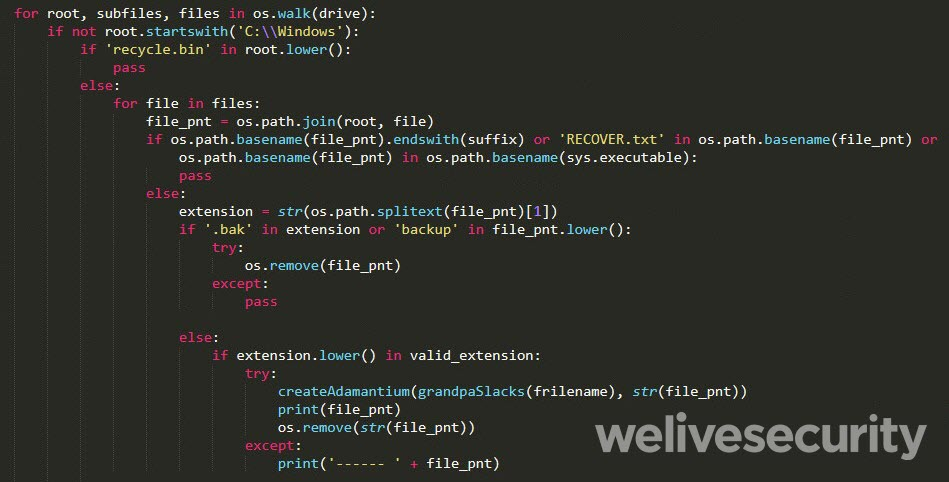
\includegraphics[height=4cm, scale=0.5]{recursos/pythonCode.png}						\end{itemize}
	\end{itemize}
\end{frame}


\begin{frame}{Tipos de Datos y Operaciones} \pause
Los programas manipulan \emph{valores} de diferentes \emph{tipos}. Por ejemplo: \pause
\begin{itemize}
	\item 1 es un valor de tipo \textbf{entero} (int).\pause
	\item 2.5 es un valor de tipo \textbf{número ``real''} (float).\pause
	\item ``hola'' es un valor de tipo \textbf{caracter} (string).\pause
	\item ``5'' es un valor de tipo \textbf{caracter} (string).\pause
	\item $[$7.0, 420, “tira de asado”$]$ es dato tipo \textbf{lista} (list).\pause	
	\item False es un valor de tipo \textbf{booleano} (bool).\pause


\begin{itemize}
\item Valores de verdad: Denotan el resultado de una evaluación lógica: los valores “verdadero” (\texttt{True}) y “falso” (\texttt{False})
\end{itemize}
\end{itemize} \pause

Los operaciones son, por ejemplo:
\begin{itemize}
	\item Suma/Resta: 3+4 $\to$ \pause 7\pause
	\item Se puede sumar strings: probar ``yo y'' + `` mi trasero''.\pause
	\item Producto: 2*8 $\to$ \pause 16\pause
	\item División: 5/2 $\to$ \pause 2.5 \pause
	\item Resto: 5\%2 $\to$ \pause 1
\end{itemize}
\end{frame}


\begin{frame}{Colab, Python, IDEs...}
\begin{block}{¿Pero qué se supone son todas esas cosas...?}\pause
\begin{itemize}
	\item Respuesta corta:\pause
		\begin{itemize}
			\item IDE = integrated development environment $\equiv$ entorno de desarrollo integrado.\pause En otras palabras, es el "soporte" sobre el cual escribiremos con el lenguaje de programación (Python, en nuestro caso) \pause
			\item Google Colab es un entorno que facilita programar en Python. Es una IDE.\pause			
			\item A su vez, Google Colab (como Anaconda, un programa usado en anteriores ediciones de este curso) nuclea un montón de paquetes o ``librerías'' (bibliotecas) para usar y no tener que andar reinventando la rueda todo el tiempo.\pause
			


		\end{itemize}
	\item Respuesta larga: nada de esto es necesario ni importante para aprender a programar o para codear en Python. Pasa más por gustos personales.\pause
	\begin{itemize}
		\item Por ejemplo, en vez de Colab o Anaconda, se podría bajar \textcolor{blue}{\href{https://www.python.org/}{Python}} e ir instalando paquetes.\pause		
		\item En vez de Colab, para codear se puede usar simplemente un editor de textos, o \textcolor{blue}{\href{https://wiki.python.org/moin/IntegratedDevelopmentEnvironments}{cualquiera de las IDEs existentes}}.
	\end{itemize}
\end{itemize}
\end{block}
\end{frame}

\begin{frame}{Lo que se viene}
\pause
\begin{center}

\includegraphics[height=7cm, scale=0.5]{recursos/meme_explosion.png}
\end{center}
\end{frame}

\begin{frame}{A codea(t)r!}
\begin{block}

\textcolor{blue}{\href{https://colab.research.google.com/drive/1pssmr5FRjDoYxt3-iadaxa-ek3ZmFwPx?usp=sharing}{Link}} a nuestra página de Google Colab	
	
\end{block}
\end{frame}


\begin{frame}{Usando Google Colab como IDE para Python}
%(IDE = integrated development environment $\equiv$ entorno de desarrollo integrado).
\begin{block}{Abriendo la IDE...}
\end{block}
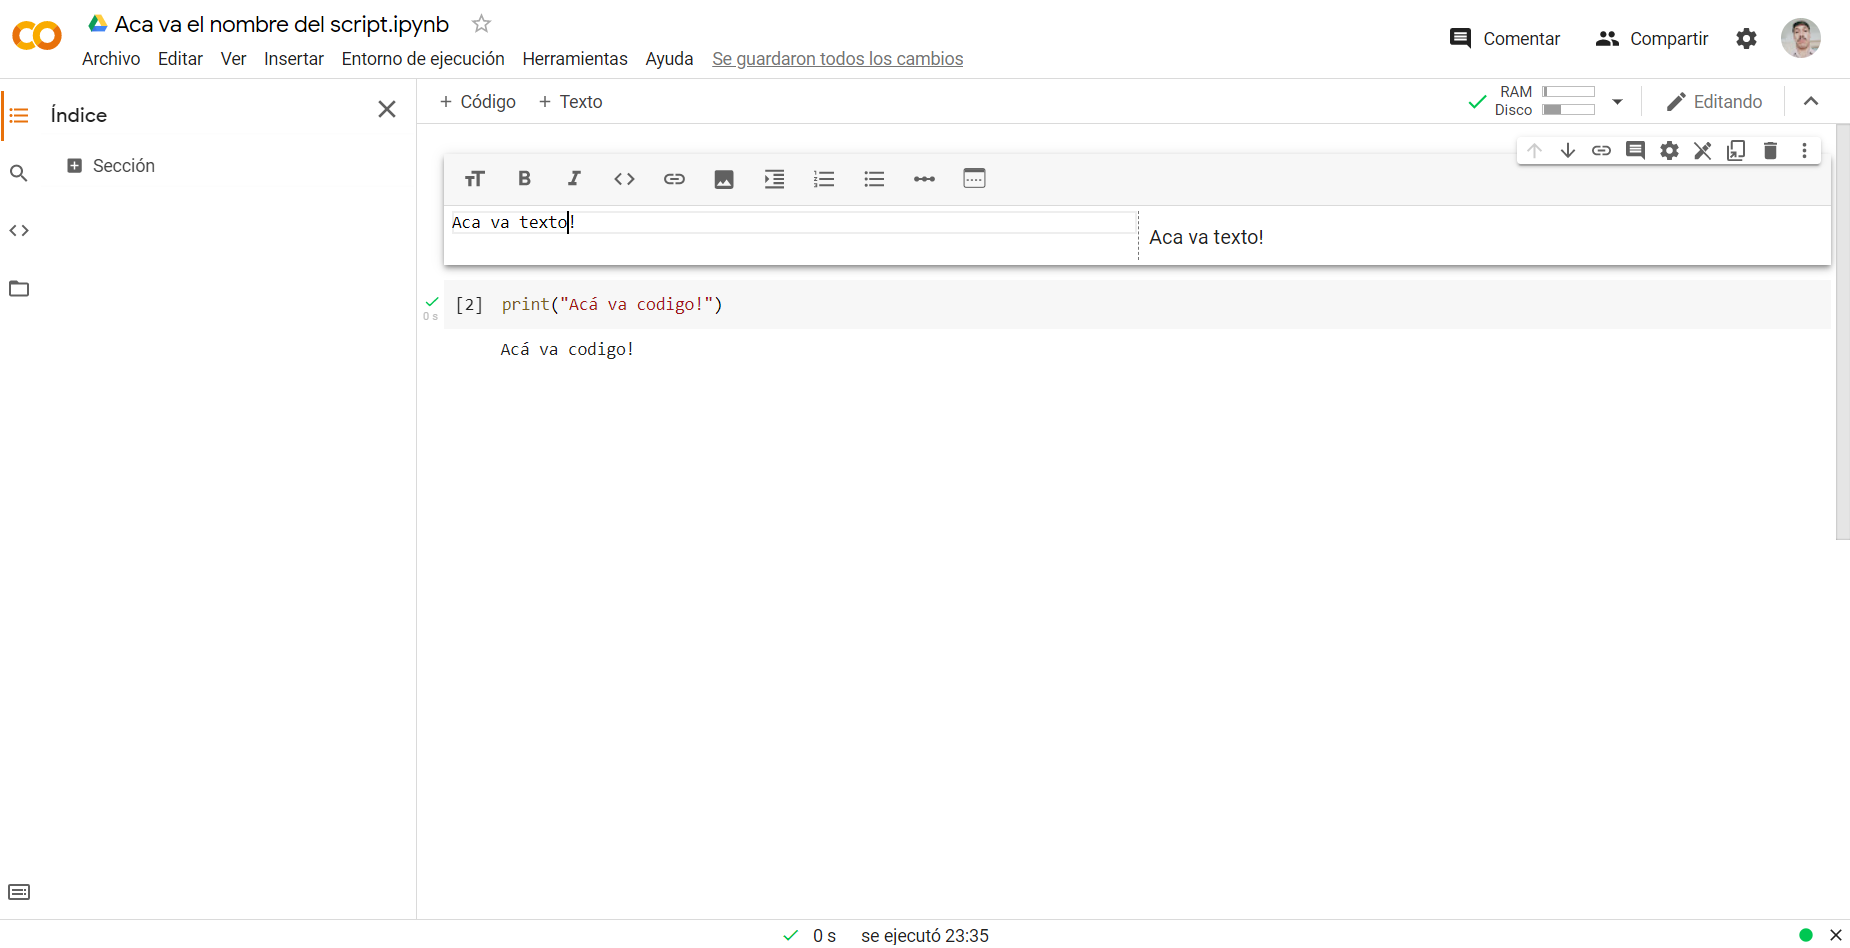
\includegraphics[scale = 0.23]{recursos/colab_raw.jpeg}
\end{frame}


\begin{frame}{Usando Google Colab como IDE para Python}
\begin{block}{Qué es cada cosa?}
\end{block}
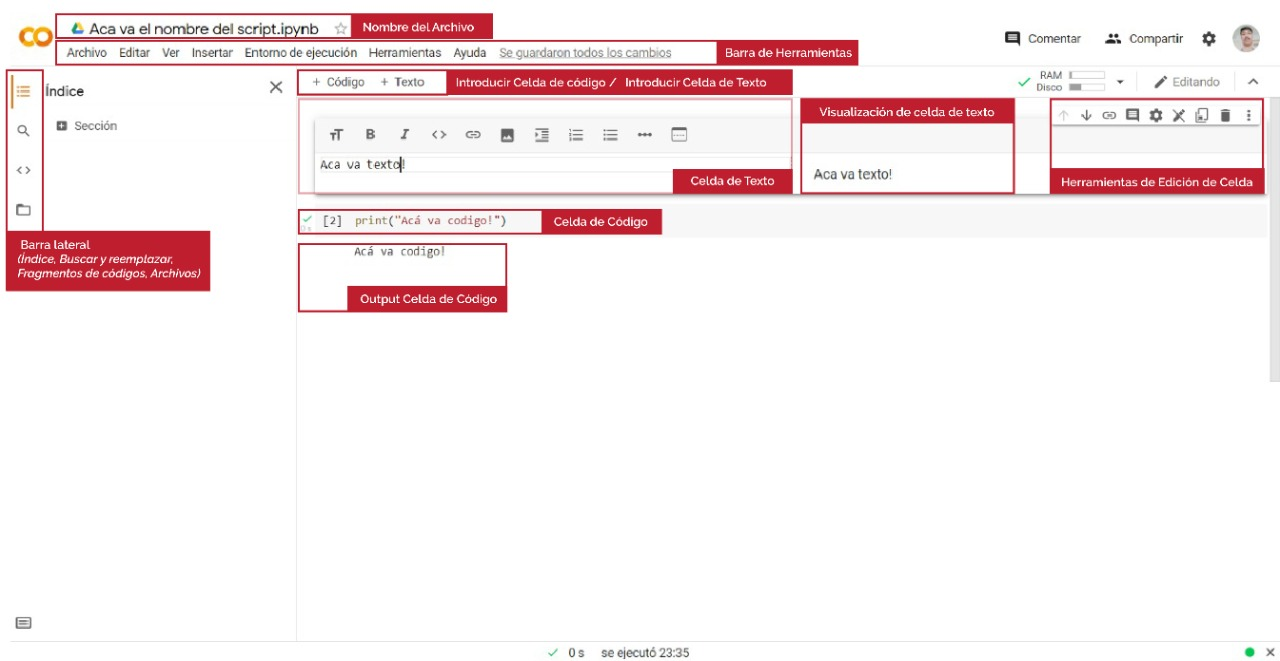
\includegraphics[scale = 0.23]{recursos/colab_edit.jpeg}
\end{frame}


\begin{frame}{Variables, expresiones y asignaciones} \pause
\begin{itemize}
	\item Una \textbf{variable} es una dirección de memoria que almacena un valor\pause
		\begin{itemize}
		\item \texttt{b = 3} asigna a la variable \texttt{b} el valor \texttt{3}\pause
		\end{itemize}
	\item Una \textbf{expresión} es una combinación de variables, valores y operadores.\pause
		\begin{itemize}
		\item \texttt{1+1} es una expresión que da como resultado \texttt{2}.\pause
		\end{itemize}
	\item Una \textbf{asignación} es una instrucción que guarda en una variable una expresión.\pause
		\begin{itemize}
		\item \texttt{long = len($[$1,3,'a'$]$)} asigna a la variable long la longitud de la lista $[$1,3,'a'$]$ \pause
		\end{itemize}
\end{itemize}
\alert{Asignación: variable = expresión}
\end{frame}


\begin{frame}{La \textbf{asignación}, nuestra primera instrucción}
\alert{VARIABLE = EXPRESIÓN} \pause
\\~
\\~
La asignación almacena el valor de la \emph{expresión} en la dirección en memoria denotada por \emph{variable} \pause
    \begin{columns}
        \begin{column}{.5\textwidth}
			\begin{itemize}
			\item \texttt{x = 1000}
           \item \texttt{x = x + 2}
			\item \texttt{x = y}
			\item \texttt{x = x + y * 22 / 33}
			\end{itemize} \pause
           
        \end{column}
        \begin{column}{.5\textwidth}\raggedleft
            
\includegraphics[scale = 0.3]{recursos/bien.png} %width=1cm,height=2cm
        \end{column}
    \end{columns}
\pause
\begin{columns}
        \begin{column}{.5\textwidth}
			\begin{itemize}
			\item \texttt{1000 = x}
           \item \texttt{x + 2 = x}
			\item \texttt{len(x) = 1}
			\end{itemize} \pause
           
        \end{column}
        \begin{column}{.5\textwidth}\raggedleft
            
\includegraphics[scale = 0.3]{recursos/mal.png} %width=1cm,height=2cm
        \end{column}
    \end{columns}
\end{frame}


\end{document}



